%% For distribution of the original source see the terms
%% for copying and modification in the file samples.dtx.
%% 
%% This generated file may be distributed as long as the
%% original source files, as listed above, are part of the
%% same distribution. (The sources need not necessarily be
%% in the same archive or directory.)
%%
%%
%% Commands for TeXCount
%TC:macro \cite [option:text,text]
%TC:macro \citep [option:text,text]
%TC:macro \citet [option:text,text]
%TC:envir table 0 1
%TC:envir table* 0 1
%TC:envir tabular [ignore] word
%TC:envir displaymath 0 word
%TC:envir math 0 word
%TC:envir comment 0 0
%%
%%
%% For submission and review of your manuscript please change the
%% command to \documentclass[manuscript, screen, review]{acmart}.
%%
%% When submitting camera ready or to TAPS, please change the command
%% to \documentclass[sigconf]{acmart} or whichever template is required
%% for your publication.
%%
%%
\documentclass[acmsmall, review, screen]{acmart}

%%
%% \BibTeX command to typeset BibTeX logo in the docs
\AtBeginDocument{%
  \providecommand\BibTeX{{%
    Bib\TeX}}}

%% Rights management information.  This information is sent to you
%% when you complete the rights form.  These commands have SAMPLE
%% values in them; it is your responsibility as an author to replace
%% the commands and values with those provided to you when you
%% complete the rights form.
\setcopyright{acmcopyright}
\copyrightyear{2022}
\acmYear{2022}
\acmDOI{XXXXXXX.XXXXXXX}

%% These commands are for a PROCEEDINGS abstract or paper.
\acmConference[Conference acronym 'XX]{Make sure to enter the correct
  conference title from your rights confirmation emai}{June 03--05,
  2018}{Woodstock, NY}
%%
%%  Uncomment \acmBooktitle if the title of the proceedings is different
%%  from ``Proceedings of ...''!
%%
%%\acmBooktitle{Woodstock '18: ACM Symposium on Neural Gaze Detection,
%%  June 03--05, 2018, Woodstock, NY}
\acmPrice{15.00}
\acmISBN{978-1-4503-XXXX-X/18/06}


%%
%% Submission ID.
%% Use this when submitting an article to a sponsored event. You'll
%% receive a unique submission ID from the organizers
%% of the event, and this ID should be used as the parameter to this command.
%%\acmSubmissionID{123-A56-BU3}

%%
%% For managing citations, it is recommended to use bibliography
%% files in BibTeX format.
%%
%% You can then either use BibTeX with the ACM-Reference-Format style,
%% or BibLaTeX with the acmnumeric or acmauthoryear sytles, that include
%% support for advanced citation of software artefact from the
%% biblatex-software package, also separately available on CTAN.
%%
%% Look at the sample-*-biblatex.tex files for templates showcasing
%% the biblatex styles.
%%

%%
%% The majority of ACM publications use numbered citations and
%% references.  The command \citestyle{authoryear} switches to the
%% "author year" style.
%%
%% If you are preparing content for an event
%% sponsored by ACM SIGGRAPH, you must use the "author year" style of
%% citations and references.
%% Uncommenting
%% the next command will enable that style.
%%\citestyle{acmauthoryear}

%% Packages
\usepackage{xcolor}
\usepackage{color}
\usepackage{listings}

%% Custom Definitions
\graphicspath{{graph/}}
\definecolor{ForestGreen}{HTML}{009B55}

\lstset{inputpath=code_examples/src/Examples}
\lstset{
  frame=none,
  xleftmargin=2pt,
  stepnumber=1,
  numbers=left,
  numbersep=5pt,
  numberstyle=\ttfamily\tiny\color[gray]{0.3},
  belowcaptionskip=\bigskipamount,
  escapeinside={*'}{'*},
  language=haskell,
  tabsize=2,
  emphstyle={\bf},
  commentstyle=\color{ForestGreen},
  stringstyle=\mdseries\rmfamily,
  showspaces=false,
  keywordstyle=\bfseries\rmfamily,
  columns=flexible,
  basicstyle=\small\sffamily,
  showstringspaces=false,
  morecomment=[l]\%,
}

%% CUSTOM PACKAGES - NON-ACCEPTED
\usepackage{todonotes}

%%
%% end of the preamble, start of the body of the document source.
\begin{document}

%%
%% The "title" command has an optional parameter,
%% allowing the author to define a "short title" to be used in page headers.
\title{LayeredTypes}
%TODO: Proper Title
%\title[LayeredTypes]{Layered Types -- A structured approach to arbitrarily combine Liquid Types}

%%
%% The "author" command and its associated commands are used to define
%% the authors and their affiliations.
%% Of note is the shared affiliation of the first two authors, and the
%% "authornote" and "authornotemark" commands
%% used to denote shared contribution to the research.
\author{Lukas Abelt}
\email{l.abelt@luabelt.de}
\orcid{1234-5678-9012}
\affiliation{%
  \institution{LASIGE}
  \streetaddress{XXX}
  \city{Lisbon}
  \state{}
  \country{Portugal}
  \postcode{}
}

%%
%% By default, the full list of authors will be used in the page
%% headers. Often, this list is too long, and will overlap
%% other information printed in the page headers. This command allows
%% the author to define a more concise list
%% of authors' names for this purpose.

%%
%% The abstract is a short summary of the work to be presented in the
%% article.
\begin{abstract}
	\todo[inline]{TODO: Abstract}
\end{abstract}

%%
%% The code below is generated by the tool at http://dl.acm.org/ccs.cfm.
%% Please copy and paste the code instead of the example below.
%% TODO
\begin{CCSXML}
<ccs2012>
 <concept>
  <concept_id>10010520.10010553.10010562</concept_id>
  <concept_desc>Computer systems organization~Embedded systems</concept_desc>
  <concept_significance>500</concept_significance>
 </concept>
 <concept>
  <concept_id>10010520.10010575.10010755</concept_id>
  <concept_desc>Computer systems organization~Redundancy</concept_desc>
  <concept_significance>300</concept_significance>
 </concept>
 <concept>
  <concept_id>10010520.10010553.10010554</concept_id>
  <concept_desc>Computer systems organization~Robotics</concept_desc>
  <concept_significance>100</concept_significance>
 </concept>
 <concept>
  <concept_id>10003033.10003083.10003095</concept_id>
  <concept_desc>Networks~Network reliability</concept_desc>
  <concept_significance>100</concept_significance>
 </concept>
</ccs2012>
\end{CCSXML}
%TODO
%\ccsdesc[500]{Computer systems organization~Embedded systems}
%\ccsdesc[300]{Computer systems organization~Redundancy}
%\ccsdesc{Computer systems organization~Robotics}
%\ccsdesc[100]{Networks~Network reliability}

%%
%% Keywords. The author(s) should pick words that accurately describe
%% the work being presented. Separate the keywords with commas.
%TODO: Keywords
\keywords{}
%% A "teaser" image appears between the author and affiliation
%% information and the body of the document, and typically spans the
%% page.
\begin{teaserfigure}
  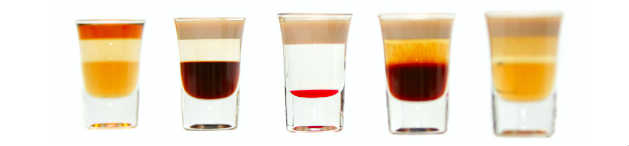
\includegraphics[width=\textwidth]{layered-shots.jpg}
  \label{fig:teaser}
  \caption{Layers in Liquids}
\end{teaserfigure}

\received{20 February 2007}
\received[revised]{12 March 2009}
\received[accepted]{5 June 2009}

%%
%% This command processes the author and affiliation and title
%% information and builds the first part of the formatted document.
\maketitle

\section{Introduction}
\subsection{Context}
Modern program languages such as C++, Haskell, Rust or Java use type systems to ensure certain promises about the correct behavior of an implementation. In essence, the type system allows the programer to specify what inputs to accept for a program or function and what outputs it will produce. While these guarantees already prevent a multitude of runtime errors, they alone cannot prevent e.g. divisions by yero or out of range accesses in arrays.

One approach to bridge this gap is the introduction of \textit{Refinement Types}, also referred to as \textit{Liquid Types}. These allow us to annotate the traditional type system with additional logical predicates in order to ensure semantic properties, which can be checked statically at compile time. Using these techniques also allows us to define pre- and post-conditions on functions' arguments and return values. By properly defining these contracts a developer can clearly communicate and moreover enforce how other developers' code is allowed to interface with their implementations. Examples for constraints might include any of the following:

\begin{itemize}
	\item Ensuring values are in certain ranges
	\item Ensuring that a list is non-empty
	\item Ensuring that data structures certain to specific semantic properties e.g. that they are sorted
\end{itemize}

All in all, refinement types are valuable building blocks to creating reliable software systems. Using them can minimize the risk of any unhandled run-time errors occuring which might lead to undesired or even undefined behavior.

\subsection{Motivation}

While Refinement Types already vastly imrpove traditional type systems, current implementations still expose some drawbacks in their practical usage. One of these challenges stems from the fact that during the static analysis, each refinement is treated as a single monolithic requirement that needs to be fulfilled. However in reality, a refinement might combine different properties of a type that may benefit from being treated individually.

One example for such a refinement in LiquidHaskell is shown in \ref{lst:combined_lt}. There, we define a function that extracts the maximum value of a (descendingly) ordered, non-empty list. In this example, this operation is equivalent to simply extracting the \texttt{head} of a list. While we only define one refinement, it actually operates on two different properties of a list. First, it imposes a restriction on it's \texttt{size} by requiring it to be non-empty, while the second restriction imposes an order on the list elements.

\lstinputlisting[firstline=6,caption={Example for a function with a combined Refinement Type in LiquidHaskell},label={lst:combined_lt}]{CombinedLT.hs}

While the refinement concerns two different aspects of the list that are independent from each other, current static analysis implementations of Liquid Types will treat it only as a single combined requirement to be fulfilled. However especially developers could benefit from a system that treats them independently: When writing code that interfaces with already existing codes such a separated approach may give a developer more fine-grained information on which requirements they still need to fulfill in their implementation.

Effectively one could treat such different requirements as separate \textit{Layers} that can be verified independently. Additionally with a proper implementation using such layers may also result in an implementation benefit, that different Layers can be defined individually and combined arbitrarily, as opposed to the example in Listing \ref{lst:combined_lt} where the combination of the two traits had to be explicitly defined as an refinement on it's own.

\subsection{Problem Definition}
\subsection{Impact}
\subsection{Approach}
\subsection{Contributions}
\section{Related Work}
\section{Background}
\section{Implementation}
\section{Evaluation}
\section{Conclusion}
\section{Acknowledgments}

\end{document}
\endinput
%%
%% End of file `sample-acmsmall-conf.tex'.
